\chapter{Fenômenos de Colisão de Partículas}
Nesse capítulo, pretendemos fazer uma introdução aos processos de colisão de
partículas e de espalhamento. Colisões de partículas consistem de um dos
métodos experimentais mais utilizados para o estudo das características da
matéria e de seus componentes. Por isso, a motivação para a melhor compreensão
desses processos é evidente.

De forma geral, os experimentos de espalhamento constituem de um bombardeamento
de um alvo por um feixe de partículas com energia bem definida. Alvos podem ser
sólidos, líquidos, gases ou outros feixes de partículas. Disso, espalhamentos
observados nesses experimentos são classificados em \textit{elásticos} e
\textit{inelásticos} a depender da excitação ou não das partículas alvo
\cite{povh6ed}. De forma resumida, no espalhamento elástico as partículas
permanecem as mesmas e não observamos decaimento ou excitação dos níveis
internos de energia. A única transferência de energia nesse caso é na forma de
energia cinética. Para uma partícula incidente $a$ atingindo uma partícula alvo
$b$ o espalhamento elástico assume a forma,
\begin{equation}
	a + b \rightarrow a' + b' .
\end{equation}
Nesse tipo de espalhamento, ambos o momento e energia são conservados (podemos
dizer que há conservação de quadrimomento). Para o espalhamento inelástico, ao
constrário, há uma alteração no nível de energia interno da partícula alvo $b$,
que, em geral, decai em outras partículas. Nesse processo pode haver liberação
de energia da estrutura interna de $b$, então podemos ter maior momento do que
começamos.
\begin{figure}[h]
	\centering
	\captionsetup{width=10cm}
	\caption{Esquemas demonstrando colisão elástica $a + b \rightarrow a' +
	b'$, e inelástica $a + b \rightarrow a' + c + d$.}
	\begin{subfigure}[b]{3.25cm}
		\centering
		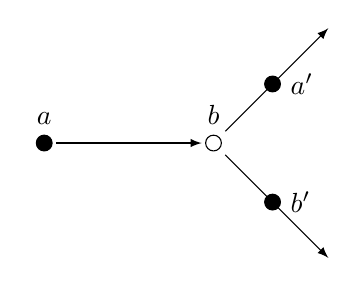
\begin{tikzpicture}[>=latex]
	\draw (-2,0) [->] -- (-0.15,0);
	\draw (0.15,0.15) [->, rotate around={45:(0.15,0.15)}] -- (2.0,0.15);
	\draw (0.15,-0.15) [->, rotate around={-45:(0.15,-0.15)}] -- (2.0,-0.15);
	\filldraw[black](-2.15,0) circle (0.1) node[above=3pt]{$a$};
	\draw (0,0) circle (0.1) node[above=3pt]{$b$};
	\filldraw (0.75,0.75) circle (0.1) node[right=3pt]{$a'$};
	\filldraw (0.75,-0.75) circle (0.1) node[right=3pt]{$b'$};
\end{tikzpicture}

	\end{subfigure}
	\hspace{1.5cm}
	\begin{subfigure}[b]{4.5cm}
		\centering
		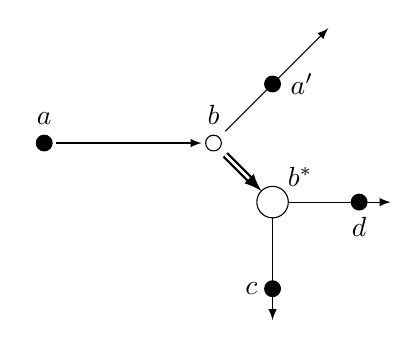
\begin{tikzpicture}[>=latex]
	\draw (-2,0) [->] -- (-0.15,0);
	\draw (0.15,0.15) [->, rotate around={45:(0.15,0.15)}] -- (2.0,0.15);
	\draw (0.15,-0.15) [
		thick, double distance=1pt, rotate around={-45:(0.15,-0.15)}, ->
	] -- (0.8,-0.15);
	\draw (0.75,-0.95)[->] -- (0.75,-2.25);
	\draw (0.95,-0.75)[->] -- (2.25,-0.75);
	\filldraw[black](-2.15,0) circle (0.1) node[above=3pt]{$a$};
	\draw (0,0) circle (0.1) node[above=3pt]{$b$};
	\filldraw (0.75,0.75) circle (0.1) node[right=3pt]{$a'$};
	\draw (0.75,-0.75) circle (0.2) node[above right=2pt]{$b^*$};
	\filldraw[black](0.75,-1.85) circle (0.1) node[left=2pt]{$c$};
	\filldraw[black](1.85,-0.75) circle (0.1) node[below=2pt]{$d$};
\end{tikzpicture}

	\end{subfigure}
\end{figure}

A medida mais útil para esse tipo de experimento é a seção de choque.  Por
seção de choque consideramos como uma quantidade experimental de interesse em
colisões \cite{griffiths_particle}.  Inicialmente, discutindo sob uma forma
clássica, podemos considerar um processo de espalhamento, no qual a partícula
entra na região de influência do centro de potencial, o qual possui parâmetro
de impacto $b$, conforme a Figura \ref{cross_section_def}. A partir da
geometria apresentada, podemos obter os seguintes diferenciais de área e ângulo
sólido, respectivamente,
\begin{gather}
d\sigma = |b\, db\, d\phi|,\\
d\Omega = |\sen \theta \, d\theta \, d\phi|.
\end{gather}
Assim, a razão entre as duas é escrita como,
\begin{equation}
\frac{d\sigma}{d\Omega} = \bigg| \frac{b}{\sen \theta} \frac{db}{d\theta}
\bigg|. \label{diff_cross_section}
\end{equation}
Aqui, assumimos que o potencial do centro de espalhamento tem simetria
azimutal, em $\phi$.

A quantidade dada na equação (\ref{diff_cross_section}) é denominada de seção
de choque diferencial \cite{griffiths_particle}.  A seção de choque total
será a seção de choque diferencial integrada sobre todo o ângulo sólido
$\Omega$ sendo ela dada por,
\begin{equation}
\sigma = \int \frac{d\sigma}{d\Omega} \sen \theta \, d\theta \, d\phi .
\end{equation}

\begin{figure}[h]
\centering
	\captionsetup{width=0.8\textwidth}
	\caption{Área diferencial $d\sigma$ indicada com centro de espalhamento
	estático com parâmetro de impacto $b$. A partícula é espalhada em um
	elemento diferencial de ângulo sólido $d\Omega$.}
\label{cross_section_def}
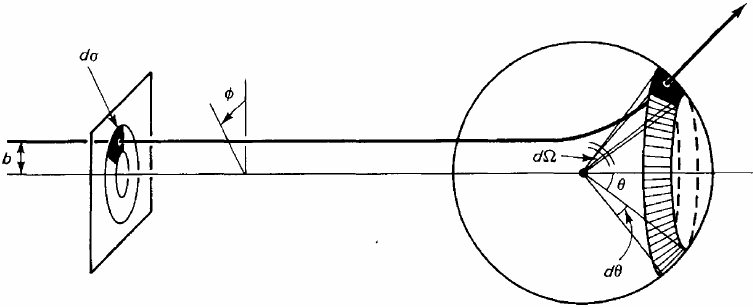
\includegraphics[width=0.8\textwidth]{./figs/cross_section.jpeg}
\fonte{Retirado de \cite{griffiths_particle}}
\end{figure}

Agora, vamos considerar um feixe de $N$ partículas monoenergéticas (de mesma
energia), todas sendo lançadas contra um dado centro de espalhamento. A
luminosidade $\mathcal{L}$ é definida como a quantidade de partícula que
atravessam a região de espalhamento por unidade de área e unidade de tempo.
Assim, a quantidade de partículas que atravessam a área $d\sigma$ por unidade
de tempo é dada por,
\begin{equation}
	dN = \mathcal{L} d\sigma.
\end{equation}
Disso segue que,
\begin{equation}
	\frac{d\sigma}{d\Omega} = \frac{1}{\mathcal{L}} \frac{dN}{d\Omega}.
\end{equation}
Essa acaba sendo uma maneira mais útil de escrevermos a seção de choque
diferencial. Sendo assim, o número de partículas espalhadas em um ângulo sólido
$dN$ dividido por $d\Omega$ e pela luminosidade.

\section{Regra de Ouro de Fermi}
A apresentação da seção de choque foi dada a partir de um ponto de vista geométrico
que, por ser simples, apresenta uma forma rápida de compreensão.


